\documentclass[t,10pt]{beamer}
\usepackage{tikz,pgfplots,pgfplotstable,pgfcalendar}

%\pgfplotstableset{col sep=comma}

\usetikzlibrary{arrows.meta}
\tikzset{>={Latex[width=7pt,length=7pt]}}
\pgfplotsset{compat=1.14}
\usepgfplotslibrary{dateplot}
\usepgfplotslibrary{units}
\usepackage{chronology}
\tikzset{eventlabel/.append style={rotate=15}}
\tikzset{every picture/.style={opacity=0.5}}
%\tikzset{chronevent/.append style={fill=darkred}}
%\usepackage{verbatim}
\usepackage{ifthen}
\usetheme{CambridgeUS}
\usefonttheme{serif}
\title{A look At The Elephant's Tail}
\author{Gregory Stark}
\date{September 14th 2016}

%\DefineVerbatimEnvironment{GitCommit}{Verbatim}{fontfamily=tt,fontsize=\small}
%\newenvironment{GitCommit}{\begin{semiverbatim}}{\end{semiverbatim}}

\newcommand{\myevent}[2]{%
  \ifthenelse{\NOT\equal{\subsecname}{}\AND\equal{\subsecname}{#2}}%
             {\tikzset{chronevent/.append style={fill=darkred}}}%
             {\tikzset{chronevent/.append style={fill=black}}}%
             \event{#1}{#2}%
}

\setbeamertemplate{footline}{
\begin{chronology}[2]{1995}{2017}{\textwidth}[0.9\textwidth]
  \myevent{\decimaldate{1}{5}{1995}}{}%Postgres95 0.1}
  \myevent{\decimaldate{25}{5}{1995}}{}%Postgres95 0.2}
  \myevent{\decimaldate{21}{7}{1995}}{}%Postgres95 0.3}
  \myevent{\decimaldate{5}{9}{1995}}{1.0}
  \myevent{\decimaldate{23}{2}{1996}}{}%Postgres95 1.01}
  \myevent{\decimaldate{1}{8}{1996}}{}%Postgres95 1.02}
  \myevent{\decimaldate{4}{11}{1996}}{}%Postgres95 1.09}
  \myevent{\decimaldate{29}{1}{1997}}{6.0}
  \myevent{\decimaldate{8}{6}{1997}}{}%6.1}
  \myevent{\decimaldate{2}{10}{1997}}{}%6.2}
  \myevent{\decimaldate{1}{3}{1998}}{6.3}
  \myevent{\decimaldate{30}{10}{1998}}{}%6.4}
  \myevent{\decimaldate{9}{6}{1999}}{6.5}
  \myevent{\decimaldate{8}{5}{2000}}{7.0}
  \myevent{\decimaldate{13}{4}{2001}}{7.1}
  \myevent{\decimaldate{4}{2}{2002}}{7.2}
  \myevent{\decimaldate{27}{11}{2002}}{7.3}
  \myevent{\decimaldate{17}{11}{2003}}{7.4}
  \myevent{\decimaldate{19}{1}{2005}}{8.0}
  \myevent{\decimaldate{8}{11}{2005}}{8.1}
  \myevent{\decimaldate{5}{12}{2006}}{8.2}
  \myevent{\decimaldate{4}{2}{2008}}{8.3}
  \myevent{\decimaldate{1}{7}{2009}}{8.4}
  \myevent{\decimaldate{20}{9}{2010}}{9.0}
  \myevent{\decimaldate{12}{9}{2011}}{9.1}
  \myevent{\decimaldate{10}{9}{2012}}{9.2}
  \myevent{\decimaldate{9}{9}{2013}}{9.3}
  \myevent{\decimaldate{18}{12}{2014}}{9.4}
  \myevent{\decimaldate{7}{1}{2016}}{9.5}
\end{chronology}
}{}

\begin{document}

\begin{frame}[plain]
  \titlepage
\end{frame}

\section{Why}
\begin{frame}{Why}
  \begin{itemize}%[<+-| alert@+>]
  \item Understanding ``who'', ``when'', and ``why'' for the decisions made
    over the past 20 years helps understand how Postgres behaves the way
    it does today including the features and limitations of the current
    code.
  \item Many of the changes fixed real problems that users faced with,
    and examining past problems helps us understand how to recognize and
    deal with problems in the future
  \item Put yourself in the shoes of an admin considering these upgrades
    and consider not just the risks of upgrading but the risks of
    \textbf{not} upgrading.
  \end{itemize}
\end{frame}


%XYZZY% \section{In the beginning}
%XYZZY% 
%XYZZY% \begin{frame}{In the beginning}
%XYZZY%   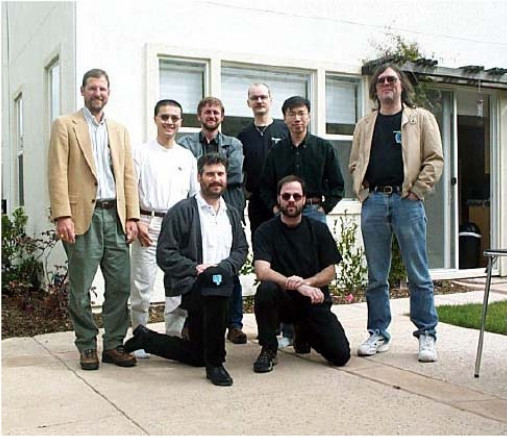
\includegraphics[width=\textwidth,height=\textheight,keepaspectratio=true]{assets/Get_to_know_PostgreSQL-6-team}
%XYZZY% \end{frame}
%XYZZY% 
%XYZZY% \begin{frame}{Postgres95 -- First Public Release}
%XYZZY%   \begin{itemize}%[<+-| alert@+>]
%XYZZY%   \item Tables limited to 1GB
%XYZZY%   \item Sorts were always on disk and always generated a new data file
%XYZZY%     for output. They always required three times as much disk space as
%XYZZY%     data being sorted
%XYZZY%   \end{itemize}
%XYZZY% \end{frame}
%XYZZY% 
%XYZZY% \begin{frame}[fragile]{Postgres 6.2 -- Use quicksort when data fits in memory}
%XYZZY%   \begin{columns}
%XYZZY%     \begin{column}{.25\textwidth}
%XYZZY%       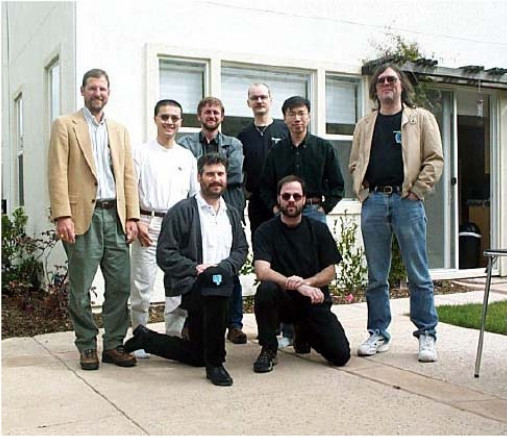
\includegraphics[width=\textwidth,height=\textheight,keepaspectratio=true]{assets/Get_to_know_PostgreSQL-6-team}
%XYZZY%     \end{column}
%XYZZY%     \begin{column}{.75\textwidth}
%XYZZY% \begin{semiverbatim}
%XYZZY% \tiny
%XYZZY%   commit 712ea2507ef7f3ea4a7149962c85de0b35245a64
%XYZZY%   Author: Vadim B. Mikheev <vadim4o@yahoo.com>
%XYZZY%   Date:   Thu Sep 18 05:37:31 1997 +0000
%XYZZY% 
%XYZZY%       1. Use qsort for first run
%XYZZY%       2. Limit number of tuples in leftist trees:
%XYZZY%           - put one tuple from current tree to disk if limit reached;
%XYZZY%           - end run creation if limit reached by nextrun.
%XYZZY%       3. Avoid mergeruns() if first run is single one!
%XYZZY% \end{semiverbatim}
%XYZZY%     \end{column}
%XYZZY%   \end{columns}
%XYZZY% \end{frame}
%XYZZY% 
%XYZZY% 
%XYZZY% %\begin{frame}{PGFPlots Bar Plot Example}
%XYZZY% %  \begin{figure}[h]
%XYZZY% %    \centering
%XYZZY% %    \begin{tikzpicture}
%XYZZY% %      \begin{axis}[
%XYZZY% %          ybar,
%XYZZY% %          enlarge x limits=0.15,
%XYZZY% %          legend style={at={(-.5,0.5)},
%XYZZY% %            anchor=north,legend columns=1},
%XYZZY% %          ylabel={\% students},
%XYZZY% %          symbolic x coords={A, B, C, D, E, F, DNF},
%XYZZY% %          xtick=data,
%XYZZY% %          bar width=2mm,
%XYZZY% %          width=0.7\textwidth
%XYZZY% %        ]
%XYZZY% %        \legend{2012, 2013};
%XYZZY% %        % Spring 2012 results
%XYZZY% %        \addplot[fill=gray]  coordinates {(A,0) (B,0) (C,3.85) (D,23.07) (E,43.31) (F,30.77) (DNF,0.00)};
%XYZZY% %        % Spring 2013 results
%XYZZY% %        \addplot[fill=blue]   coordinates {(A,0) (B,3.70) (C,22.22) (D,22.22) (E,40.74) (F,3.70) (DNF,7.41)};
%XYZZY% %      \end{axis}
%XYZZY% %    \end{tikzpicture}
%XYZZY% %    \caption{Consistent improvement over the last year}
%XYZZY% %  \end{figure}
%XYZZY% %\end{frame}
%XYZZY% 

\section{Experiments}
\subsection{}
\begin{frame}{Line Chart of pivot table}
Here is a chart:

  \begin{tikzpicture}
  \begin{axis}[
      height=.50\textheight,
      width=.50\textwidth,
      title=Performance over time for various number of clients,
      xlabel=GIT Commit Date,
      ylabel=Transactions/s,
      grid=major,
      date coordinates in=x,
      mark size=0.25pt,
      scaled ticks=false,
      yticklabel style={
        /pgf/number format/fixed,
        font=\tiny,
      },
      xticklabel style={
        rotate=-30,
        anchor=west,
        %draw=black,
        font=\tiny,
      },
      xticklabel={\year-\month-\day},
      xmin=1995-01-01,
      xmax=2017-01-01]
    \addplot table[col sep=comma,header=true,x index=0,y=4] {pivot-table.csv};
    \addplot table[col sep=comma,header=true,x index=0,y=8] {pivot-table.csv};
    \addplot table[col sep=comma,header=true,x index=0,y=12] {pivot-table.csv};
    \addplot table[col sep=comma,header=true,x index=0,y=16] {pivot-table.csv};
    \addplot table[col sep=comma,header=true,x index=0,y=20] {pivot-table.csv};
    \addplot table[col sep=comma,header=true,x index=0,y=24] {pivot-table.csv};
    \addplot table[col sep=comma,header=true,x index=0,y=28] {pivot-table.csv};
    \addplot table[col sep=comma,header=true,x index=0,y=40] {pivot-table.csv};
    \addplot table[col sep=comma,header=true,x index=0,y=56] {pivot-table.csv};
    \addplot table[col sep=comma,header=true,x index=0,y=72] {pivot-table.csv};
    \addplot table[col sep=comma,header=true,x index=0,y=80] {pivot-table.csv};
    \addplot table[col sep=comma,header=true,x index=0,y=88] {pivot-table.csv};
  \end{axis}
\end{tikzpicture}

There was a chart
\end{frame}


\section{In The Beginning}
\subsection{1.0}
\begin{frame}{Postgres95 1.0}
  \begin{itemize}%[<+-| alert@+>]
  \item The copyright of Postgres 1.0 has been loosened to be freely
    modifiable and modifiable for any purpose.  Please read the
    COPYRIGHT file.  Thanks to Professor Michael Stonebraker for making
    this possible.
  \item pg\_dump - a utility for dumping out a postgres database into
    a script file containing query commands. The script files are in
    an ASCII format and can be used to reconstruct the database, even
    on other machines and other architectures. (Also good for
    converting a Postgres 4.2 database to Postgres95 database.)
  \item The SQL statement for creating a database is `CREATE DATABASE' instead
    of `CREATEDB'. Similarly, dropping a database is `DROP DATABASE' instead
    of `DESTROYDB'. However, the names of the executables `createdb' and
    `destroydb' remain the same.
  \end{itemize}
\end{frame}
\subsection{1.0}
\begin{frame}{PostgreSQL 6.0}
  \begin{itemize}%[<+-| alert@+>]
  \item Name change from Postgres95 to PostgreSQL
  \end{itemize}
\end{frame}
\subsection{6.3}
\begin{frame}{PostgreSQL 6.2}
  \begin{itemize}%[<+-| alert@+>]
  \item The regression tests have been adapted and extensively modified for the 6.1 release of PostgreSQL.
  \item Allow internal sorts to be stored in memory rather than in files (Bruce \& Vadim)
  \item Triggers implemented with CREATE TRIGGER (SQL3)(Vadim)
  \item SPI (Server Programming Interface) allows execution of queries inside C-functions (Vadim)
  \end{itemize}
\end{frame}
\begin{frame}{PostgreSQL 6.3}
  \begin{itemize}%[<+-| alert@+>]
  \item Many new SQL features, including full SQL92 subselect capability (everything is here but target-list subselects).
  \item New SQL statement CREATE PROCEDURAL LANGUAGE(Jan)
  \item We also have real deadlock detection code. No more sixty-second timeouts.
  \end{itemize}
\end{frame}
\subsection{6.5}
\begin{frame}{PostgreSQL 6.5}
  \begin{itemize}%[<+-| alert@+>]
  \item Multiversion concurrency control(MVCC)
  \item Hot backups from pg\_dump
  \end{itemize}
\end{frame}


\section{Early production use}
\subsection{7.0}
\begin{frame}{PostgreSQL 7.0}
  \begin{itemize}%[<+-| alert@+>]
  \item Foreign keys are now implemented... Many users have been asking for this feature, and we are pleased to offer it.
  \item SQL92 join syntax is now supported, though only as INNER JOIN for this release. 
  \end{itemize}
\end{frame}
\subsection{7.1}
\begin{frame}{PostgreSQL 7.1}
  \begin{itemize}%[<+-| alert@+>]
  \item Write-ahead Log (WAL)
  \item TOAST
  \item Outer Joins
  \item The previous C function manager did not handle null values properly, nor did it support 64-bit CPU's (Alpha)
  \end{itemize}
\end{frame}
\subsection{7.2}
\begin{frame}{PostgreSQL 7.2}
  \begin{itemize}%[<+-| alert@+>]
  \item Vacuuming no longer locks tables, thus allowing normal user access during the vacuum.
  \item There is no longer a problem with installations that exceed four billion transactions.
  \item The system now computes histogram column statistics during ANALYZE, allowing much better optimizer choices.
  \item Program and library messages can now be displayed in several languages.
  \end{itemize}
\end{frame}
\subsection{7.3}
\begin{frame}{PostgreSQL 7.3}
  \begin{itemize}%[<+-| alert@+>]
  \item PostgreSQL now supports the ALTER TABLE ... DROP COLUMN functionality.
  \item Both multibyte and locale support are now always enabled.
  \end{itemize}
\end{frame}
\subsection{7.4}
\begin{frame}{PostgreSQL 7.4}
  \begin{itemize}%[<+-| alert@+>]
  \item New client-to-server protocol
  \item New autovacuum tool
  \item IN / NOT IN subqueries are now much more efficient
  \item Improved GROUP BY processing by using hash buckets
  \end{itemize}
\end{frame}


\section{Scaling up}
\subsection{8.0}
\begin{frame}{PostgreSQL 8.0}
  \begin{itemize}%[<+-| alert@+>]
  \item Microsoft Windows Native Server
  \item Point-In-Time Recovery
  \item Tablespaces
  \item Savepoints
  \end{itemize}
\end{frame}
\subsection{8.1}
\begin{frame}{PostgreSQL 8.1}
  \begin{itemize}%[<+-| alert@+>]
  \item Allow index scans to use an intermediate in-memory bitmap (Tom)
  \item Add shared row level locks using SELECT ... FOR SHARE (Alvaro)
  \item Improve performance for partitioned tables (Simon) (Constraint Exclusion)
  \item Skip WAL logging for CREATE TABLE AS / SELECT INTO (Simon)
  \end{itemize}
\end{frame}
\subsection{8.2}
\begin{frame}{PostgreSQL 8.2}
  \begin{itemize}%[<+-| alert@+>]
  \item Index creation without blocking concurrent INSERT/UPDATE/DELETE operations
  \item Improved sorting performance with lower memory usage
  \item Easier administration of warm standby servers
  \end{itemize}
\end{frame}
\subsection{8.3}
\begin{frame}{PostgreSQL 8.3}
  \begin{itemize}%[<+-| alert@+>]
  \item Using non-persistent transaction IDs for read-only transactions reduces overhead and VACUUM requirements
  \item Heap-Only Tuples (HOT) accelerate space reuse for most UPDATEs and DELETEs
  \item Checkpoint writes can be spread over a longer time period to smooth the I/O spike during each checkpoint
  \item Just-in-time background writer strategy improves disk write efficiency
  \item Support multiple concurrent autovacuum processes, and other autovacuum improvements
  \end{itemize}
\end{frame}
\begin{frame}{Table Bloat}
  \begin{tikzpicture}
    \begin{axis}[
      height=.75\textheight,
      width=0.9\textwidth,
      title=Table Bloat over time,
      xlabel=Time (hours),
      ylabel=Size of pgbench\_accounts Table (kB),
      grid=major,
      mark size=0,
      scaled ticks=false,
      xmin=0,ymin=0,
      enlargelimits=false,
      yticklabel style={
        /pgf/number format/fixed,
        font=\tiny,
      },
      xtick distance=1,
      xticklabel style={
        /pgf/number format/fixed,
        font=\tiny,
      },
      legend entries={7.3, 7.4, 8.0, 8.1, 8.2, 8.3, 8.4, 9.0, 9.1, 9.2, 9.3, 9.4, 9.5},
      ]
      \addplot table[]{du.out.2008-01-03-REL7_3_21};
      \addplot table[]{du.out.2010-10-01-REL7_4_30};
      \addplot table[]{du.out.2010-10-01-REL8_0_26};
      \addplot table[]{du.out.2010-12-13-REL8_1_23};
      \addplot table[]{du.out.2011-12-01-REL8_2_23};
      \addplot table[]{du.out.2013-02-04-REL8_3_23};
      \addplot table[]{du.out.2014-07-21-REL8_4_22};
      \addplot table[]{du.out.2015-10-05-REL9_0_23};
      \addplot table[]{du.out.2015-10-05-REL9_1_19};
      \addplot table[]{du.out.2015-10-05-REL9_2_14};
      \addplot table[]{du.out.2015-10-05-REL9_3_10};
      \addplot table[]{du.out.2015-10-05-REL9_4_5};
      \addplot table[]{du.out.2016-01-04-REL9_5_0};
    \end{axis}
  \end{tikzpicture}
\end{frame}

\subsection{8.4}
\begin{frame}{PostgreSQL 8.4}
  \begin{itemize}%[<+-| alert@+>]
  \item Visibility Map
  \item Free Space Map
  \item Windowing Functions
  \item Common Table Expressions and Recursive Queries
  \end{itemize}
\end{frame}

\section{New frontiers}
\subsection{9.0}
\begin{frame}{PostgreSQL 9.0}
  \begin{itemize}%[<+-| alert@+>]
  \item Streaming Replication, allowing continuous archive (WAL) files to be streamed over a network connection to a standby server
  \item Hot Standby, allowing continuous archive standby servers to execute read-only queries
  \item pg\_upgrade to support in-place upgrades from 8.3 or 8.4 to 9.0.
  \end{itemize}
\end{frame}
\subsection{9.1}
\begin{frame}{PostgreSQL 9.1}
  \begin{itemize}%[<+-| alert@+>]
  \item Synchronous Replication
  \item Foreign Tables
  \item Per-Column Collation Support
  \item True Serializable Isolation Level
  \item Unlogged Tables
  \end{itemize}
\end{frame}
\subsection{9.2}
\begin{frame}{PostgreSQL 9.2}
  \begin{itemize}%[<+-| alert@+>]
  \item Index-Only Scans
  \item Cascading Replication
  \item Allow pg\_basebackup to make base backups from standby servers
  \item Add a JSON data type
  \end{itemize}
\end{frame}
\subsection{9.3}
\begin{frame}{PostgreSQL 9.3}
  \begin{itemize}%[<+-| alert@+>]
  \item Materialized views
  \item Make simple views auto-updatable
  \item Allow foreign data wrappers to support writes (inserts/updates/deletes) on foreign tables
  \end{itemize}
\end{frame}
\subsection{9.4}
\begin{frame}{PostgreSQL 9.4}
  \begin{itemize}%[<+-| alert@+>]
  \item Add jsonb, a more capable and efficient data type for storing JSON data
  \item Add new SQL command ALTER SYSTEM for changing postgresql.conf configuration file entries
  \item Allow materialized views to be refreshed without blocking concurrent reads
  \item Add support for logical decoding of WAL data, to allow database changes to be streamed out in a customizable format
  \end{itemize}
\end{frame}
\subsection{9.5}
\begin{frame}{PostgreSQL 9.5}
  \begin{itemize}%[<+-| alert@+>]
  \item Allow INSERTs that would generate constraint conflicts to be turned into UPDATEs or ignored
  \item Add row-level security control
  \item Add Block Range Indexes (BRIN)
  \item Substantial performance improvements for sorting
  \item Substantial performance improvements for multi-CPU machines
  \end{itemize}
\end{frame}
\subsection{9.6}
\begin{frame}{PostgreSQL 9.6}
  \begin{itemize}%[<+-| alert@+>]
  \item Parallel execution of sequential scans, joins and aggregates
  \item postgres\_fdw now supports remote joins, sorts, UPDATEs, and DELETEs
  \item Substantial performance improvements, especially in the area of scalability on multi-CPU-socket servers
  \end{itemize}
\end{frame}

\section{The future}
\begin{frame}{PostgreSQL 10}
  \begin{itemize}%[<+-| alert@+>]
  \item Parallel Sort?
  \item Multi-master Logical Replication?
  \item Autonomous Transactions?
  \end{itemize}
\end{frame}

\end{document}
